\documentclass[11pt,a4paper]{article}
\usepackage[utf8]{inputenc}
\usepackage[french]{babel}
\usepackage[T1]{fontenc}

\usepackage{amsmath}
\usepackage{amsfonts}
\usepackage{amssymb}

\newcommand{\NomAuteur}{Fabrice BOISSIER}
\newcommand{\TitreMatiere}{Architecture des Ordinateurs}
\newcommand{\NomUniv}{EPITA - Bachelor Cyber Sécurité}
\newcommand{\NiveauUniv}{CYBER1}
\newcommand{\NumGroupe}{CYBER1}
\newcommand{\AnneeUniv}{ }
\newcommand{\DateExam}{18 novembre 2022}
\newcommand{\TypeExam}{CORRECTION Examen (Sujet 2)}
\newcommand{\TitreExam}{\TitreMatiere}
\newcommand{\DureeExam}{1h30}
\newcommand{\MyWaterMark}{\AnneeUniv} % Watermark de protection

% Ajout de mes classes & definitions
\usepackage{MetalExam} % Appelle un .sty

% "Tableau" et pas "Table"
\addto\captionsfrench{\def\tablename{Tableau}}

%%%%%%%%%%%%%%%%%%%%%%%
%Header
%%%%%%%%%%%%%%%%%%%%%%%
\lhead{\TypeExam}							%Gauche Haut
\chead{\NomUniv}							%Centre Haut
\rhead{\NumGroupe}							%Droite Haut
\lfoot{\DateExam}							%Gauche Bas
\cfoot{\thepage{} / \pageref*{LastPage}}	%Centre Bas
\rfoot{\texttt{\TitreMatiere}}				%Droite Bas

%%%%%

\usepackage{tabularx}

\newlength{\LabelWidth}%
%\setlength{\LabelWidth}{1.3in}%
\setlength{\LabelWidth}{1cm}%
%\settowidth{\LabelWidth}{Employee E-mail:}%  Specify the widest text here.

% Optional first parameter here specifies the alignment of
% the text within the \makebox.  Default is [l] for left
% alignment. Other options are [r] and [c] for right and center
\newcommand*{\AdjustSize}[2][l]{\makebox[\LabelWidth][#1]{#2}}%


\definecolor{mGreen}{rgb}{0,0.6,0}
\definecolor{mGray}{rgb}{0.5,0.5,0.5}
\definecolor{mPurple}{rgb}{0.58,0,0.82}
\definecolor{backgroundColour}{rgb}{0.95,0.95,0.92}

\lstdefinestyle{CStyle}{
    backgroundcolor=\color{backgroundColour},
    commentstyle=\color{mGreen},
    keywordstyle=\color{magenta},
    numberstyle=\tiny\color{mGray},
    stringstyle=\color{mPurple},
    basicstyle=\footnotesize,
    breakatwhitespace=false,
    breaklines=true,
    captionpos=b,
    keepspaces=true,
    numbers=left,
    numbersep=5pt,
    showspaces=false,
    showstringspaces=false,
    showtabs=false,
    tabsize=2,
    language=C
}


\hyphenation{op-tical net-works SIGKILL}


\begin{document}

%\MakeExamTitleDuree     % Pour afficher la duree
\MakeExamTitle                   % Ne pas afficher la duree

%% \MakeStudentName    %% A reutiliser sur chaque nouvelle page

\bigskip
%\bigskip

Vous devez respecter les consignes suivantes, sous peine de 0 :

\begin{itemize}
\item Lisez le sujet en entier avec attention
\item Répondez sur le sujet
\item Ne détachez pas les agrafes du sujet
\item \'Ecrivez lisiblement vos réponses (si nécessaire en majuscules)
\item Les appareils électroniques sont tous interdits (calculatrices également)
\item Ne trichez pas
\end{itemize}

%\bigskip

\vfillFirst

% Questions cours
\section{Questions (10 points)}

\subsection{(1 point) Rappelez les 14 premières puissances de 2 : }

\bigskip


\begin{table}[ht!]
\centerline{
\begin{tabular}{ | m{0.5cm} | m{0.5cm} | m{0.5cm} | m{0.5cm} | m{0.65cm} | m{0.65cm} | m{0.65cm} | m{1cm} | m{1cm} | m{1cm} | m{1.5cm} | m{1.5cm} | m{1.5cm} | m{1.5cm} |}
\hline
$ 2^{0} $ & $ 2^{1} $ & $ 2^{2} $ & $ 2^{3} $ & $ 2^{4} $ & $ 2^{5} $ & $ 2^{6} $ & $ 2^{7} $ & $ 2^{8} $ & $ 2^{9} $ & $ 2^{10} $ & $ 2^{11} $ &  $ 2^{12} $ &  $ 2^{13} $ \\
\hline
 & & & & & & & & & & & & & \\
 1 & 2 & 4 & 8 & 16 & 32 & 64 & 128 & 256 & 512 & 1024 & 2048 & 4096 & 8192 \\
 & & & & & & & & & & & & & \\
\hline
\end{tabular}
}
\end{table}


\bigskip

\subsection{(3 points) Convertissez ces nombres en décimaux. Vous donnerez leur interprétation non-signée puis signée.}

\bigskip

\centerline{
\begin{tabular}{ c |  m{2cm}   c   m{2cm} | m{2cm}   c   m{2cm} }
                                & & non-signé & & & signé & \\
 & & & &  & & \\
\hline
 & & & &  & & \\
$ \% \, 1000 \; 1011 \; 0101 $  & &  2229  & & &  -1867  & \\
 & & & &  & & \\
\hline
 & & & &  & & \\
$ \% \, 1011 \; 1100 \; 1110 $  & &  3022  & & &  -1074  & \\
 & & & &  & & \\
\hline
 & & & &  & & \\
$ \% \, 1001 \; 1010 \; 0011 $  & &  2467  & & &  -1629  & \\
 & & & &  & & \\
\hline
 & & & &  & & \\
\$ DEF  & &   3567  & & &  -529   & \\
 & & & &  & & \\
\hline
 & & & &  & & \\
\$ 86A  & &   2154  & & &  -1942  & \\
 & & & &  & & \\
\hline
 & & & &  & & \\
\$ E86  & &   3718  & & &  -378  & \\
 & & & &  & & \\
\end{tabular}
}

% \bigskip

\vfillLast

\newpage

\subsection{(4 points) Convertissez ces nombres décimaux en binaire sur 8 bits ou 12 bits, puis en hexadécimal.}

\bigskip

\centerline{
\begin{tabular}{ c |  m{2cm}   c   m{2cm} | m{2cm}   c   m{2cm} }
                                & & binaire & & & hexadécimal & \\
 & & & &  & & \\
\hline
 & & & &  & & \\
$ 42 $    & & \% 0010 1010        & & &  \$ 2A  & \\
 & & & &  & & \\
\hline
 & & & &  & & \\
$ 1258 $  & & \% 0100 1110 1010   & & &  \$ 4EA  & \\
 & & & &  & & \\
\hline
 & & & &  & & \\
$ 324 $   & & \% 0001 0100 0100   & & &  \$ 144  & \\
 & & & &  & & \\
\hline
 & & & &  & & \\
$ -86 $   & & \% 1010 1010        & & &  \$ AA  & \\
 & & & &  & & \\
\end{tabular}
}

\bigskip

\bigskip

\subsection{(2 points) Convertissez ces nombres en flottants au format IEEE 754 simple précision : }

\bigskip

\centerline{
\begin{tabular}{ c |  m{1.75cm}   c   m{1.75cm} | m{1.75cm}   c   m{1.75cm} }
                                & & exposant & & & hexadécimal & \\
 & & & &  & & \\
\hline
 & & & &  & & \\
$ 67,109375 $   & &  133 / \% 1000 0101  & & &  \$ 4286 3800  & \\
 & & & &  & & \\
\hline
 & & & &  & & \\
$ -82,1015625 $ & &  133 / \% 1000 0101  & & &  \$ C2A4 3400  & \\
 & & & &  & & \\
\end{tabular}
}


\bigskip

\bigskip

\bigskip

%%%%%%%%%%%%%%%%%%%%%%%%%%%%%%%%%%%%%%%%%%%%%%%%%%%%%%%
%%%%%%%%%%%%%%%%%%%%%%%%%%%%%%%%%%%%%%%%%%%%%%%%%%%%%%%
%%%%%%%%%%%%%%%%%%%%%%%%%%%%%%%%%%%%%%%%%%%%%%%%%%%%%%%

\section{Problème (10 points)}


Un étudiant en cybersécurité faisant ses premières expériences en \textit{forensic} (analyse forensique ou investigation numérique en français) a besoin de vous pour convertir plusieurs valeurs et retrouver des informations.
Celui-ci a récupéré un disque dur qui servait dans un RAID 1, et il souhaite retrouver les noms de fichiers, le contenu de ces fichiers, mais également analyser quelques programmes stockés dessus.

\bigskip

\subsection{(2 points) Première étape : lecture d'une structure }

L'étudiant a réussi à extraire un secteur du disque dur formaté en FAT16 qui contenait une liste de fichiers et l'identifiant unique associé.
Il a isolé 2 \textit{direntries}, les a affiché en hexadécimal, et vous demande de séparer les champs.
Utilisez le modèle de structure d'une \textit{direntry} pour séparer les différentes données et remplir les tableaux suivants avec les valeurs hexadécimales.

\newpage

\begin{table}[ht!]
  \centering
  \begin{minipage}{0.45\textwidth}
    \centering
% %*   *)
% [style=algorithmique]
\begin{lstlisting}[language=C]
struct direntry {
  char[11] name;
  char     attributes;
  int      first_cluster;
  long     size;
} __attribute__((packed)) \end{lstlisting}
  \end{minipage}
  \hfillx
  \begin{minipage}{0.45\textwidth}
Les types de données font :

\begin{itemize}
\item char : 1 octet (8 bits)
\item int : 2 octets (16 bits)
\item long : 4 octets (32 bits)
\end{itemize}

\textit{Rappel : char[11] correspond à un tableau de 11 cases (de 0 à 10)}
  \end{minipage}
%  \caption{Algorithme de la somme des N premiers entiers}
%  \label{somme-n-premiers-entiers}
\end{table}





\begin{table}[ht!]
  \centering
  \begin{minipage}{0.3\textwidth}
    \centering
% %*   *)
%\begin{lstlisting}[style=algorithmique]
%direntry 1 :
%00 00 00 50 4F 55
%45 54 54 58 54 1F
%00 14 00 00 00 12
%
%direntry 2 :
%00 00 00 50 49 45
%44 53 41 56 49 1F
%00 32 00 00 31 55
%\end{lstlisting}

\centering{
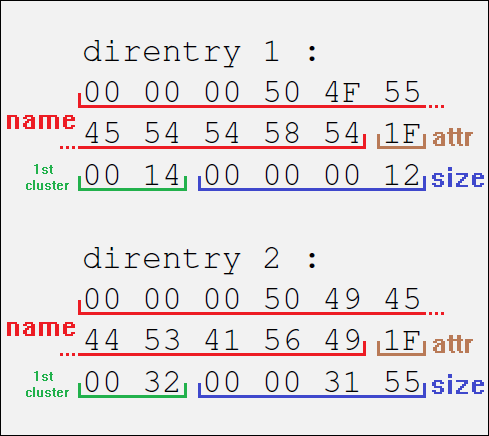
\includegraphics[scale=0.42]{img/Tab_Sujet_2_underlined.png}
}

  \end{minipage}
  \hfillx
  \begin{minipage}{0.65\textwidth}
    \centering

\begin{tabular}{ | c | C{4cm} | C{4cm} | }
\hline
 & direntry 1 (f1) & direntry 2 (f2) \\
\hline
 & & \\
name &  00 00 00 50 4F 55 45 54 54 58 54  &  00 00 00 50 49 45 44 53 41 56 49  \\
 & & \\
\hline
 & & \\
attributes &  1F  &  1F  \\
 & & \\
\hline
 & & \\
first\_cluster &  00 14  &  00 32  \\
 & & \\
\hline
 & & \\
size &  00 00 00 12  &  00 00 31 55  \\
 & & \\
\hline
\end{tabular}

  \end{minipage}
%  \caption{Algorithme de la somme des N premiers entiers}
%  \label{somme-n-premiers-entiers}
\end{table}

%\bigskip

\subsection{(2 points) Deuxième étape : conversion des noms }

L'étudiant semble dubitatif et vous demande de lui présenter des valeurs lisibles.
Pour cela, il vous fournit une toute petite table de conversion ASCII... mais vous vous apercevez qu'il n'a pas du tout recopié la partie la plus essentielle de la table (probablement car il ne prenait pas assez de notes) : sa table ne dispose que de la correspondance entre des caractères et leurs valeurs en base 10.
Il vous faut donc convertir les valeurs hexadécimales à la main (zut alors).

\medskip

Concernant les noms de fichiers, la norme FAT16 précise que sur les caractères, les 8 premiers servent à coder le nom du fichier, et les 3 derniers servent à coder l'extension.
Vous devez donc ajouter un point pour séparer l'extension du nom de fichier.

\medskip

\begin{table}[ht!]
  \centering
  \begin{minipage}{0.3\textwidth}
    \centering

\begin{tabular}{ |c|c| m{0.3cm} |c|c| }
\cline{1-2} \cline{4-5}
Dec & Char &   & Dec & Char \\
\cline{1-2} \cline{4-5}
48 & 0 &  & 49 & 1 \\
\cline{1-2} \cline{4-5}
65 & A &  & 78 & N \\
66 & B &  & 79 & O \\
67 & C &  & 80 & P \\
68 & D &  & 81 & Q \\
69 & E &  & 82 & R \\
70 & F &  & 83 & S \\
71 & G &  & 84 & T \\
72 & H &  & 85 & U \\
73 & I &  & 86 & V \\
74 & J &  & 87 & W \\
75 & K &  & 88 & X \\
76 & L &  & 89 & Y \\
77 & M &  & 90 & Z \\
\cline{1-2} \cline{4-5}
\end{tabular}

  \end{minipage}
  \hfillx
  \begin{minipage}{0.65\textwidth}
    \centering

\begin{tabular}{ c   | m{0.45cm} | m{0.45cm} | m{0.45cm} | m{0.45cm} | m{0.45cm} | m{0.45cm} | m{0.45cm} | m{0.45cm} | c | m{0.45cm} | m{0.45cm} | m{0.45cm} | }
\cline{2-9} \cline{11-13}
 & & & & & & & & &   & & & \\
f1   & & & &  P  &  O  &  U  &  E  &  T  &  .  &  T  &  X  &  T  \\
 & & & & & & & & &   & & & \\
\cline{2-9} \cline{11-13}
 & & & & & & & & &   & & & \\
f2   & & & &  P  &  I  &  E  &  D  &  S  &  .  &  A  &  V  &  I  \\
 & & & & & & & & &   & & & \\
\cline{2-9} \cline{11-13}
\end{tabular}

  \end{minipage}
%  \caption{Algorithme de la somme des N premiers entiers}
%  \label{somme-n-premiers-entiers}
\end{table}


%\bigskip

\newpage

\subsection{(2 points) Troisième étape : conversion des champs }

L'étudiant commence à avoir confiance en vous : vous avez trouvé les bons noms de fichiers (et il reconnait les noms).
Afin de pouvoir vous donner les bons clusters à lire, il vous demande de convertir cette fois la taille contenu dans les champs de chaque direntry, ainsi que le numéro du premier cluster, en nombre décimaux (afin qu'il puisse les mettre en paramètre de son outil d'extraction).

\smallskip

\begin{center}
\begin{tabular}{ | c | C{5cm} | C{7.5cm} | }
\hline
 & taille du fichier & numéro du premier cluster \\
\hline
 & & \\
direntry 1 (f1) &  18  &  20  \\
 & & \\
\hline
 & & \\
direntry 2 (f2) &  12629  &  50  \\
 & & \\
\hline
\end{tabular}
\end{center}

\smallskip

\subsection{(2 points) Quatrième étape : lecture d'un fichier }

L'étudiant est surexcité, vous êtes sur le point de l'aider à retrouver des fichiers et leurs contenus !
En récupérant la vidéo, l'étudiant vous répond qu'il ne peut pas vous la montrer car celle-ci \textit{serait} corrompue.
Néanmoins, tout a l'air correct pour le fichier texte.

\smallskip

Il vous demande de convertir maintenant le contenu du fichier en ASCII, et si possible, de retrouver le numéro codé en binaire dans ce texte.

\begin{table}[ht!]
  \centering
  \begin{minipage}{0.3\textwidth}
    \centering

% %*   *)
\begin{lstlisting}[style=algorithmique]
46 4C 41 47 30 31
30 30 31 31 31 30
\end{lstlisting}

  \end{minipage}
  \hfillx
  \begin{minipage}{0.3\textwidth}
    \centering

texte :

\medskip

\begin{tabular}{ | m{2.5cm} | }
\hline
 \\ \\ %\\
FLAG 01001110
 \\ \\ \\
\hline
\end{tabular}

  \end{minipage}
  \hfillx
  \begin{minipage}{0.3\textwidth}
    \centering

numéro :

\medskip

\begin{tabular}{ | m{2.5cm} | }
\hline
 \\ \\ \\
68
 \\ \\ \\
\hline
\end{tabular}

  \end{minipage}
%  \caption{Algorithme de la somme des N premiers entiers}
%  \label{somme-n-premiers-entiers}
\end{table}

%\smallskip

\subsection{(2 points) Cinquième étape : désassemblage }

L'étudiant n'en croit pas ses yeux : vous avez démontré que vous méritez votre bachelor en cybersécurité.
Il vous demande d'utiliser vos talents de \texttt{h4x0rz} pour désassembler des instructions et les analyser.
L'étudiant vous indique qu'il a mis 3 instructions \texttt{MOV}, mais il ne se souvient plus de leur ordre.
En vous aidant de la documentation fournie, indiquez l'ordre (par 1, 2, ou 3).

\bigskip

\centering{
\begin{tabular}{ | c | c | c | }
\hline
Opcode & Instruction & Description \\
\hline
88 & MOV r/m8, r8   & Déplace une valeur d'un registre 8 bits vers un registre ou une adresse \\
8A & MOV r8, r/m8   & Déplace une valeur 8 bits vers un registre 8 bits \\
8B & MOV r32, r/m32 & Déplace une valeur 32 bits vers un registre 32 bits \\
\hline
\end{tabular}
}

\smallskip

\begin{table}[ht!]
  \centering
  \begin{minipage}{0.55\textwidth}
    \centering

% %*   *)
\begin{lstlisting}[style=algorithmique]
[1]  401c2d:   88 3c 25 16 00 00 00
[2]  401c3b:   8a 24 25 16 00 00 00
[3]  401c34:   8b 1c 25 99 55 64 16
\end{lstlisting}

  \end{minipage}
  \hfillx
  \begin{minipage}{0.4\textwidth}
    \centering

\begin{tabular}{ | m{1cm} | c |}
\hline
 & \\
2 & \texttt{mov    0x16,\%ah} \\
 & \\
\hline
 & \\
1 & \texttt{mov    \%bh,0x16} \\
 & \\
\hline
 & \\
3 & \texttt{mov    0x16645599,\%ebx} \\
 & \\
\hline
\end{tabular}

  \end{minipage}
%  \caption{Algorithme de la somme des N premiers entiers}
%  \label{somme-n-premiers-entiers}
\end{table}

\bigskip

\end{document}
